\documentclass[pra,12pt]{revtex4-2}
\usepackage{amsmath}
\usepackage{amssymb}
\usepackage{graphicx}
\usepackage{color}
\usepackage{mathrsfs}
\usepackage{enumerate}
\usepackage{epigraph}
\usepackage{framed}
\usepackage[pdfborder={0 0 0},colorlinks=true,linkcolor=blue,urlcolor=blue]{hyperref}

\def\ket#1{\left|#1\right\rangle}
\def\bra#1{\left\langle#1\right|}
\def\braket#1{\left\langle#1\right\rangle}
\def\hvbox[#1]#2{\,\boxed{\scalebox{0.7}{$\,#1$}|\scalebox{0.7}{$#2\,$}}}

\usepackage{fancyhdr}
\fancyhf{}
\lhead{\tiny Y.~D.~Chong}
\rhead{\scriptsize Ch.~3: Quantum Entanglement $|$ Graduate Quantum Mechanics}
\lfoot{}
\rfoot{\thepage}
\pagestyle{fancy}

\setlength{\parindent}{14pt}
\setlength{\fboxsep}{0.01\fboxsep}
\renewcommand{\theequation}{3.\arabic{equation}}

\renewcommand{\baselinestretch}{1.0}
\setlength{\parskip}{0.04in}

\def\thesection{3.\arabic{section}}
\def\thesubsection{3.\arabic{section}.\arabic{subsection}}

\begin{document}
\setcounter{page}{36}

\begin{center}
{\Large \textbf{Chapter 3: Quantum Entanglement}}
\end{center}

\epigraph{They don't think it be like it is, \\but it do.}{Oscar Gamble}

\section{Quantum states of multi-particle systems}

So far, we have studied quantum mechanical systems consisting of
single particles; the next important step is to consider systems of
multiple particles.  As we shall see, applying the postulates of
quantum mechanics to multi-particle systems leads to many important
and counterintuitive phenomena, such as \textbf{quantum entanglement}.

\subsection{Tensor products}
\label{sec:tensorprod}

Suppose we have two quantum objects, $A$ and $B$.  According to
quantum mechanics, $A$ is associated with some Hilbert space
$\mathscr{H}_A$ (meaning that every state of A is a vector in that
space), and $B$ is similarly associated with a Hilbert space
$\mathscr{H}_B$.  Note that $\mathscr{H}_A$ and $\mathscr{H}_B$ may be
mathematically distinct; for example, they may have different
dimensions.  Now, the combined system of $A$ and $B$ should likewise
be describable by quantum mechanics.  What is its Hilbert space?

In linear algebra, there is an concept called the \textbf{tensor
  product} which turns out to be exactly what we need to answer this
question.  Given $|a\rangle \in \mathscr{H}_A$ and $|b\rangle \in
\mathscr{H}_B$, consider an ordered pair of these two vectors, which
we call ``the tensor product of $|a\rangle$ and $|b\rangle$'', and
which we denote by
\begin{equation*}
  |a\rangle \otimes |b\rangle.
\end{equation*}
Note that this is an \textit{ordered} pair, i.e.,
$|a\rangle\otimes|b\rangle$ is not necessarily the same as
$|b\rangle\otimes|a\rangle$.

It turns out that tensor products can act as vectors: they can form
linear combinations, by addition to each other and/or multiplication
by scalars (complex numbers).  These vector operations are related to
the original vector operations for $\mathscr{H}_A$ and $\mathscr{H}_B$
via a pair of ``factorization rules'',
\begin{align}
  \Big(\lambda |a\rangle
  + \lambda' |a'\rangle\Big) \otimes |b\rangle &=
  \lambda |a\rangle \otimes |b\rangle \,+\,
  \lambda' |a'\rangle \otimes |b\rangle, \label{tensorrule1} \\
  |a\rangle \otimes \Big(\lambda |b\rangle
  + \lambda' |b'\rangle\Big) &=
  \lambda |a\rangle \otimes |b\rangle \,+\,
  \lambda' |a\rangle \otimes |b'\rangle.
  \label{tensorrule2} 
\end{align}
These are reminiscent of the rules of ordinary algebra, with $\otimes$
acting like multiplication (except that $|a\rangle\otimes|b\rangle \ne
|b\rangle\otimes|a\rangle$ in general).

We will be dealing with tensor products a lot, and it can be
cumbersome to keep writing the $\otimes$.  Therefore, it is customary
to simplify by omitting the $\otimes$ in bra-ket notation:
\begin{equation}
  |a \rangle \otimes |b\rangle \;\; \equiv \;\; |a \rangle |b\rangle.
\end{equation}
However, the ordering is always retained: whenever we see such a
``product of two kets'', the vector on the left is always understood
to be the $A$-type vector in the tensor product, and the one on the
right is the $B$-type vector.

It can be shown that the space of all tensor products, \textit{and
  linear combinations thereof}, forms a Hilbert space.  We call this
the tensor product space of $\mathscr{H}_A$ and $\mathscr{H}_B$,
denoted by
\begin{equation*}
  \mathscr{H}_A\otimes \mathscr{H}_B.
\end{equation*}
(For denoting tensor product \textit{spaces}, we will not omit the
$\otimes$ symbol.)  The tensor product thus provides a natural way to combine two Hilbert spaces to form a larger Hilbert space.

As an explicit example, let both $\mathscr{H}_A$ and $\mathscr{H}_B$
be the space of two-component complex vectors, $\mathbb{C}^2$.  Given
two vectors
\begin{equation}
  |a\rangle = \begin{pmatrix} a_1 \\ a_2 \end{pmatrix} \in \mathbb{C}^2,
  \quad
  |b\rangle = \begin{pmatrix} b_1 \\ b_2 \end{pmatrix} \in \mathbb{C}^2,
\end{equation}
we can define the tensor product as
\begin{equation}
  |a\rangle |b\rangle =
  \begin{pmatrix} a_1 b_1 \\ a_1 b_2 \\ a_2 b_1 \\ a_2 b_2 \end{pmatrix}.
  \label{tensordef}
\end{equation}
This is a vector in the space of four-component complex vectors,
$\mathbb{C}^4$, which serves as the tensor product space.  From
Eq.~\eqref{tensordef}, it is clear that $|a\rangle \otimes |b\rangle
\ne |b\rangle \otimes |a\rangle$ in general.  We can also show that
Eq.~\eqref{tensordef} satisfies the factorization rules
\eqref{tensorrule1}--\eqref{tensorrule2}.  For instance,
\begin{align}
  \left[\begin{pmatrix} a_1 \\ a_2 \end{pmatrix}
    + \begin{pmatrix} a_1' \\ a_2' \end{pmatrix} \right]
  \otimes \begin{pmatrix} b_1 \\ b_2 \end{pmatrix}
  &=
  \begin{pmatrix} (a_1+a_1') b_1 \\ (a_1+a_1') b_2 \\
    (a_2+a_2') b_1 \\ (a_2+a_2') b_2 \end{pmatrix} \\
  &=
  \begin{pmatrix} a_1 b_1 \\ a_1 b_2 \\ a_2 b_1 \\ a_2 b_2 \end{pmatrix}
  + \begin{pmatrix} a_1' b_1 \\ a_1' b_2 \\ a_2' b_1 \\ a_2' b_2 \end{pmatrix}\\
  &= \begin{pmatrix} a_1 \\ a_2 \end{pmatrix} \otimes
  \begin{pmatrix} b_1 \\ b_2 \end{pmatrix}
  + \begin{pmatrix} a_1' \\ a_2' \end{pmatrix} \otimes
  \begin{pmatrix} b_1 \\ b_2 \end{pmatrix}.
\end{align}
We can calculate inner products between tensor products in a pretty
straightforward way.  The dual of Eq.~\eqref{tensordef} is
\begin{equation}
  \langle a| \langle b| =
  \begin{pmatrix} a_1^* b_1^* & a_1^* b_2^*
    & a_2^* b_1^* & a_2^* b_2^* \end{pmatrix}.
\end{equation}
(Note that taking the dual does not affect the ordering of the tensor
product.)  Hence,
\begin{align}
  \Big(\langle a| \langle b|\Big)
  \Big(|a'\rangle |b'\rangle\Big)
  &= \begin{pmatrix} a_1^* b_1^* & a_1^* b_2^*
    & a_2^* b_1^* & a_2^* b_2^* \end{pmatrix}
  \begin{pmatrix} a_1' b_1' \\ a_1' b_2' \\
    a_2' b_1' \\ a_2' b_2' \end{pmatrix} \label{inprodex1}\\
  &= (a_1^*a_1' + a_2^*a_2') (b_1^*b_1' + b_2^*b_2') \\
  &= \langle a|a'\rangle \; \langle b|b'\rangle.  
  \label{inprodex3}
\end{align}
The inner product is performed ``slot by slot'', by taking the inner
products of the original $A$-type and $B$-type vectors, and
multiplying the resulting numbers.  It can be shown that this
procedure preserves the inner product axioms.

The key features of the above example generalize to more complicated
tensor products, including cases where $\mathscr{H}_A$ and
$\mathscr{H}_B$ are inequivalent (e.g., when they have different
dimensions).  To proceed, let us suppose the two vector spaces have
orthonormal bases, possibly of different sizes, denoted like this:
\begin{align}
  \Big\{ |\alpha\rangle \Big\} &\;\;\textrm{is a basis for}\;\; \mathscr{H}_A,
  \;\mathrm{where}\;\; \alpha = 1, 2, \dots, \mathrm{dim}(\mathscr{H}_A)\\
  \Big\{ |\beta\rangle \Big\} &\;\; \textrm{is a basis for}\;\; \mathscr{H}_B,
  \;\mathrm{where}\;\; \beta\, = 1, 2, \dots, \mathrm{dim}(\mathscr{H}_B).
\end{align}
Given that $\mathscr{H}_A \otimes \mathscr{H}_B$ is defined as the
space of all possible tensor products and their linear combinations,
we can see that
\begin{align}
  \Big\{ |\alpha \rangle |\beta \rangle \Big\}
  \;\;\textrm{is a basis for}\;\; \mathscr{H}_A \otimes \mathscr{H}_B,
  \;\mathrm{where}\;
  \begin{cases}
    \alpha &= 1, 2, \dots, \mathrm{dim}(\mathscr{H}_A), \\
    \beta &= 1, 2, \dots, \mathrm{dim}(\mathscr{H}_B).
  \end{cases}
\end{align}
This basis is orthonormal because, as in
Eqs.~\eqref{inprodex1}--\eqref{inprodex3},
\begin{equation}
  \Big(\langle \alpha| \langle \beta|\Big)
  \Big(|\alpha'\rangle |\beta'\rangle\Big)
  = \langle \alpha|\alpha'\rangle \; \langle \beta|\beta'\rangle
  = \delta_{\alpha\alpha'} \delta_{\beta\beta'}.
  \label{innerprod}
\end{equation}
Hence,
\begin{equation}
  \dim\left[\mathscr{H}_A \otimes \mathscr{H}_B\right]
  = \mathrm{dim}(\mathscr{H}_A)\; \mathrm{dim}(\mathscr{H}_B).
  \label{tensordim}
\end{equation}

Returning to the earlier $\mathbb{C}^2\otimes\mathbb{C}^2$ example,
let us take the following orthonormal basis for both $\mathscr{H}_A =
\mathbb{C}^2$ and $\mathscr{H}_B = \mathbb{C}^2$:
\begin{equation}
  |\!\uparrow\rangle = \begin{pmatrix}1 \\ 0 \end{pmatrix}, \quad
  |\!\downarrow\rangle = \begin{pmatrix}0 \\ 1 \end{pmatrix}.
\end{equation}
In a quantum mechanical context, $A$ and $B$ could each represent a
spin-$1/2$ subsystem, with $|\!\uparrow\rangle$ denoting the spin-up
state and $|\!\downarrow\rangle$ the spin-down state (e.g., along the
$z$ axis).  Then, using Eq.~\eqref{tensordef}, we find that
\begin{align}
  \begin{aligned}
  |\!\uparrow\rangle  |\!\uparrow\rangle
  &= \begin{pmatrix}1 \\ 0 \\ 0 \\ 0\end{pmatrix},\quad
  |\!\uparrow\rangle  |\!\downarrow\rangle
  = \begin{pmatrix}0 \\ 1 \\ 0 \\ 0\end{pmatrix}, \\
  |\!\downarrow\rangle  |\!\uparrow\rangle
  &= \begin{pmatrix}0 \\ 0 \\ 1 \\ 0\end{pmatrix},\quad
  |\!\downarrow\rangle  |\!\downarrow\rangle
  = \begin{pmatrix}0 \\ 0 \\ 0 \\ 1\end{pmatrix}.
  \end{aligned}
\end{align}
This is, of course, an orthonormal basis for the tensor product space
$\mathbb{C}^2\otimes\mathbb{C}^2 = \mathbb{C}^4$, which is the state
space for the combined system of two spins.

\subsection{Entanglement}

The above definition of the tensor product space contains an important
subtlety.  Even though we used tensor products of the form
\begin{equation}
  |a\rangle |b\rangle
  \label{tprod_generic}
\end{equation}
to help define the tensor product space, vectors drawn from
$\mathscr{H}_A \otimes \mathscr{H}_B$ do not necessarily have this
form.  This is because $\mathscr{H}_A \otimes \mathscr{H}_B$ is the
space formed by tensor products \textit{and their linear
  combinations}.

In quantum mechanics, tensor products like \eqref{tprod_generic} are
the natural way to describe a situation where subsystem $A$ has a
quantum state $|a\rangle$, and $B$ has a quantum state $|b\rangle$.
For example, suppose each of them represents a spin-$1/2$ subsystem,
with $|\!\uparrow\rangle$ denoting the spin-up state and
$|\!\downarrow\rangle$ denoting the spin-down state (along the $z$
axis).  If $A$ and $B$ are both in the spin-up state, then the state
of combined system is, naturally,
\begin{equation}
  |\!\uparrow\rangle |\!\uparrow\rangle.
  \label{stateexample1}
\end{equation}
Similarly, suppose the states of $A$ and $B$ are
\begin{align}
  \begin{aligned}
  |a\rangle &= |\!\uparrow\rangle,\\
  |b\rangle &= \frac{1}{\sqrt{2}}
  \Big(|\!\uparrow\rangle + |\!\downarrow\rangle\Big).
  \end{aligned}
\end{align}
Then the state of the combined system is
\begin{align}
  |a\rangle\, |b\rangle
  = |\!\uparrow\rangle\, \frac{1}{\sqrt{2}}\,
  \Big(|\!\uparrow\rangle + |\!\downarrow\rangle\Big)
  = \frac{1}{\sqrt{2}} \Big( |\!\uparrow\rangle \, |\!\uparrow\rangle
  + |\!\uparrow\rangle\, |\!\downarrow\rangle \Big).
  \label{stateexample2}
\end{align}

But let us consider the state vector
\begin{equation}
  |\psi\rangle = \frac{1}{\sqrt{2}}
  \Big(|\!\uparrow\rangle\, |\!\downarrow\rangle
  \,-\, |\!\downarrow\rangle \, |\!\uparrow\rangle\Big).
  \label{entangled_state}
\end{equation}
Evidently, just like \eqref{stateexample1} and \eqref{stateexample2},
this is a valid vector in $\mathscr{H}_A \otimes \mathscr{H}_B =
\mathbb{C}^2\otimes\mathbb{C}^2$.  But unlike \eqref{stateexample1}
and \eqref{stateexample2}, it turns out that there is no way to write
\eqref{entangled_state} in the form $|a\rangle|b\rangle$!  (We will
prove this later, in Section~\ref{sec:entropy}.)  In such a situation,
each of $A$ and $B$ cannot be said to have a stand-alone quantum
state; only the combined system possesses a well-defined quantum state
$|\psi\rangle$.  The two subsystems are said to be \textbf{entangled}.

Quantum entanglement leads to many counterintuitive phenomena, which
will be explored in the rest of this chapter.

\subsection{Multiple subsystems}

The above tensor product formalism can be straightforwardly extended
to the case of more than two subsystems.

Suppose a quantum system has $N$ subsystems with Hilbert spaces
$\mathscr{H}_1, \mathscr{H}_2, \dots, \mathscr{H}_N$.  Then the
combined system is described by the Hilbert space
\begin{equation}
  \mathscr{H}_1 \otimes \mathscr{H}_2 \otimes \cdots \otimes
  \mathscr{H}_N,
\end{equation}
which has dimension
\begin{equation}
  \mathrm{dim}\left[\mathscr{H}_1 \otimes \cdots \otimes \mathscr{H}_N\right]
  = \mathrm{dim}\left[\mathscr{H}_1\right] \cdot
  \mathrm{dim}\left[\mathscr{H}_2\right] \cdots
  \mathrm{dim}\left[\mathscr{H}_N\right].
\end{equation}
It is remarkable that the dimension scales exponentially with the
number of subsystems.  For instance, if there are 20 subsystems each
having a 2D Hilbert space, then the combined Hilbert space has
dimension $2^{20} =1\,048\,576$.  Thus, quantum systems with only a
modest number of particles can carry tremendous amounts of information
in their quantum states.  This is one of the motivations behind the
active research fields of quantum computing and quantum information
theory.

%% By the way, the tensor product plays a role even in the quantum
%% mechanics of a particle moving in multiple spatial dimensions, even if
%% this was not emphasized in introductory courses.  For instance, in 2D
%% space the position is determined by two coordinates (e.g., $x$ and
%% $y$), so each position eigenstate is actually a tensor product:
%% \begin{equation*}
%%   |\,\mathbf{r} = (x,y)\,\rangle \;\equiv\; |x\rangle\otimes
%%   |y\rangle.
%% \end{equation*}

If the subsystems in question are particles, we assume for now that
the particles are distinguishable.  There are other complications that
arise if the particles are ``identical'', which will be the subject of
the next chapter (if you're unsure what this means, just read on).

\section{Partial measurements}
\label{sec:partialmeasurements}

Let us recall how measurements work in single-particle quantum theory.
Each observable $Q$ is described by some Hermitian operator $\hat{Q}$,
which has an eigenbasis $\{|q_i\rangle\}$ such that
\begin{equation}
  \hat{Q}|q_i\rangle = q_i |q_i\rangle.
\end{equation}
For simplicity, let the eigenvalues $\{q_i\}$ be non-degenerate.
Suppose a particle initially has quantum state $|\psi\rangle$.  This
can always be expanded in terms of the eigenbasis of $\hat{Q}$:
\begin{equation}
  |\psi\rangle = \sum_i \psi_i\, |q_i\rangle, \;\;\mathrm{where}\;\;\,\textrm{and}\;\, \psi_i = \langle q_i|\psi\rangle.
\end{equation}
The \textbf{measurement postulate of quantum mechanics} states that if
we measure $Q$, then (i) the probability of obtaining the measurement
outcome $q_i$ is $P_i = |\psi_i|^2$, the absolute square of the
coefficient of $|q_i\rangle$ in the basis expansion; and (ii) upon
obtaining this outcome, the system instantly ``collapses'' into state
$|q_i\rangle$.

Mathematically, these two rules can be summarized using the projection
operator
\begin{equation}
  \hat{\Pi}(q_i) = |q_i\rangle\langle q_i|.
\end{equation}
Applying this operator to $|\psi\rangle$ gives the non-normalized
state vector
\begin{equation}
  |\psi'\rangle = |q_i\rangle \langle q_i|\psi\rangle.
\end{equation}
From this, we glean two pieces of information:
\begin{itemize}
\item The probability of obtaining this outcome is
  $\langle\psi'|\psi'\rangle = |\langle q_i|\psi\rangle|^2$.

\item The post-collapse state is obtained by the re-normalization
  $|\psi'\rangle \rightarrow |q_i\rangle$.
\end{itemize}

For multi-particle systems, there is a new complication: what if a
measurement is performed on just one particle?

Consider a system of two particles A and B, with two-particle Hilbert
space $\mathscr{H}_A \otimes \mathscr{H}_B$.  We perform a measurement
on particle $A$, corresponding to a Hermitian operator $\hat{Q}_A$
that acts upon $\mathscr{H}_A$ and has eigenvectors $\{|\mu\rangle\;
|\; \mu = 1, 2, \dots\}$ (i.e., the eigenvectors are enumerated by
some index $\mu$).  We can write any state $|\psi\rangle$ using the
eigenbasis of $\hat{Q}_A$ for the $\mathscr{H}_A$ part, and an
arbitrary basis $\{|\nu\rangle\}$ for the $\mathscr{H}_B$ part:
\begin{align}
  \begin{aligned}
    |\psi\rangle &= \sum_{\mu\nu}
    \psi_{\mu\nu}\, |\mu\rangle |\nu\rangle \\
    &= \sum_\mu |\mu\rangle |\varphi_\mu \rangle,
    \;\;\;\mathrm{where}\;\;\;
    |\varphi_\mu\rangle\equiv \sum_\nu \psi_{\mu\nu}\,|\nu\rangle
    \;\in\; \mathscr{H}_B.
  \end{aligned}
  \label{psi_twop}
\end{align}
Unlike the single-particle case, the ``coefficient'' of
$|\mu_i\rangle$ in this basis expansion is not a complex number, but a
vector in $\mathscr{H}_B$.

Proceeding by analogy, the probability of obtaining the outcome
labelled by $\mu$ should be the ``absolute square'' of this
``coefficient'', $\langle\varphi_\mu|\varphi_\mu\rangle$.  Let us
define the partial projector
\begin{equation}
  \hat{\Pi}(\mu) \,=\, |\mu\rangle\langle \mu| \otimes  \hat{I}.
\end{equation}
The $A$ slot of this operator contains a projector,
$|\mu\rangle\langle \mu|$, while the $B$ slot leaves the
$\mathscr{H}_B$ part of the two-particle space unchanged.  Applying
the partial projector to the state given in Eq.~\eqref{psi_twop} gives
\begin{equation}
  |\psi'\rangle \,=\, \hat{\Pi}(\mu)\, |\psi\rangle
  \,=\, |\mu\rangle |\varphi_\mu\rangle.
\end{equation}
Now we follow the same measurement rules as before.  The outcome
probability is
\begin{equation}
  P_\mu = \langle\psi'|\psi'\rangle
  = \langle \mu|\mu\rangle\, \langle \varphi_\mu|\varphi_\mu\rangle
  = \sum_\nu |\psi_{\mu\nu}|^2.
\end{equation}
The post-measurement collapsed state is obtained by the
re-normalization
\begin{equation}
  |\psi'\rangle
  \;\;\rightarrow\;\;
  \frac{1}{\sqrt{\sum_{\nu'} |\psi_{\mu\nu'}|^2}}\;
  \sum_{\nu} \psi_{\mu\nu} |\mu\rangle |\nu\rangle.
\end{equation}

\begin{framed}
\noindent
\textit{Example}---A system of two spin-$1/2$ particles is in
the ``singlet state''
\begin{equation}
  |\psi\rangle = \frac{1}{\sqrt{2}} \Big(|\!+\!z\rangle|\!-\!z\rangle \,-\, |\!-\!z\rangle|\!+\!z\rangle\Big).
\end{equation}
For each particle, $|\!+\!z\,\rangle$ and $|\!-\!z\,\rangle$ denote
eigenstates of the operator $\hat{S}_z$, with eigenvalues $+\hbar/2$
and $-\hbar/2$ respectively.  Suppose we measure $S_z$ on particle A.
What are the probabilities of the possible outcomes, and the
associated post-collapse states?

\begin{itemize}
\item \textbf{First outcome: $+\hbar/2$}.
  \begin{itemize}
  \item The partial projector is $|\!+\!z\rangle\langle+z| \otimes \hat{I}$.
  \item Applying the projection to $|\psi\rangle$ yields
    $|\psi'\rangle = (1/\sqrt{2})\,|\!+\!z\rangle|\!-\!z\rangle$.
  \item The outcome probability is $\displaystyle
    P_+ = \langle \psi'|\psi'\rangle = \frac{1}{2}$.
  \item The post-collapse state is $\displaystyle
    \frac{1}{\sqrt{P_+}} |\psi'\rangle = |\!+\!z\rangle |\!-\!z\rangle$
  \end{itemize}

\item \textbf{Second outcome: $-\hbar/2$}.
  \begin{itemize}
  \item The partial projector is $|\!-\!z\rangle\langle-z| \otimes
    \hat{I}$.
  \item Applying the projection to $|\psi\rangle$ yields
    $|\psi'\rangle = (1/\sqrt{2})\,|\!-\!z\rangle|\!+\!z\rangle$.
  \item The outcome probability is $\displaystyle P_- = \langle \psi'|\psi'\rangle =
    \frac{1}{2}$.
  \item The post-collapse state is $\displaystyle = \frac{1}{\sqrt{P_-}} |\psi'\rangle
    = |\!-\!z\rangle |\!+\!z\rangle$.
  \end{itemize}
\end{itemize}
The two possible outcomes, $+\hbar/2$ and $-\hbar/2$, occur with equal
probability.  In either case, the two-particle state collapses so that
$A$ is in the observed spin eigenstate, and $B$ has the opposite spin.
After the collapse, the two-particle state is no longer entangled.
\end{framed}

\section{The Einstein-Podolsky-Rosen ``paradox''}

In 1935, Einstein, Podolsky, and Rosen (EPR) formulated a thought
experiment, now known as the \textbf{EPR paradox}, that highlights the
counter-intuitive features of quantum entanglement [\ref{cite:epr}].
They tried to use this thought experiment to argue that quantum theory
cannot serve as a fundamental description of reality.  Subsequently,
however, it was shown that the EPR paradox is not an actual paradox;
physical systems \textit{really do} have the strange behavior that the
thought experiment highlighted.

Consider an entangled state, like the following ``singlet state'' of
two spin-$1/2$ particles:
\begin{equation}
  |\psi\rangle = \frac{1}{\sqrt{2}} \Big(|\!+\!z\rangle|\!-\!z\rangle \,-\, |\!-\!z\rangle|\!+\!z\rangle\Big).
  \label{eprsinglet}
\end{equation}
As before, let the two particles be labeled $A$ and $B$.  Measuring
$S_z$ on $A$ collapses the system into a two-particle state that is
unentangled, where each particle has a definite spin.  If the
measurement outcome is $+\hbar/2$, the new state is $|\!+\!z\rangle
|\!-\!z\rangle$, whereas if the outcome is $-\hbar/2$, the new state
is $|\!-\!z\rangle|\!+\!z\rangle$.

The postulates of quantum theory seem to indicate that the state
collapse happens instantaneously, regardless of the distance
separating the particles.  Imagine that we prepare the two-particle
state in a laboratory on Earth.  Particle $A$ is then transported to
the laboratory of Alice, in the Alpha Centauri star system, and
particle $B$ is transported to the laboratory of Bob, in the
Betelgeuse system, separated by $\sim 640$ light years.  In principle,
this can be done carefully enough to avoid disturbing the two-particle
quantum state.

\begin{figure}[h]
  \centering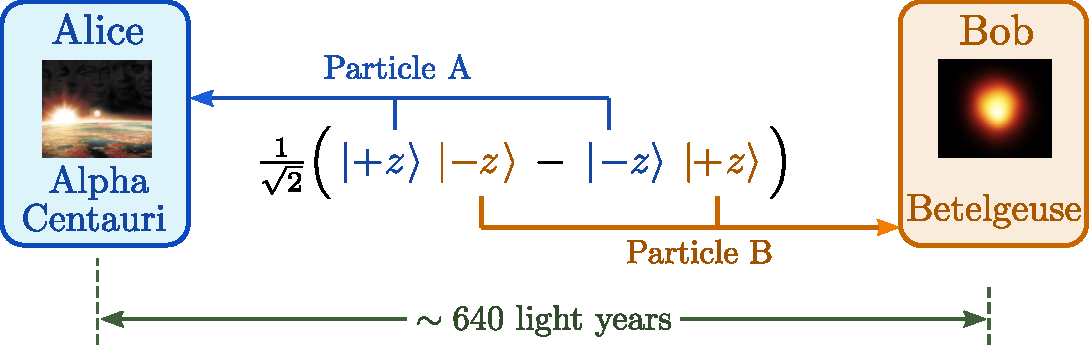
\includegraphics[width=0.75\textwidth]{epr}
\end{figure}

Once ready, Alice measures $\hat{S}_z$ on particle $A$, which induces
an instantaneous collapse of the two-particle state.  Immediately
afterwards, Bob measures $\hat{S}_z$ on particle $B$, and
obtains---with 100\% certainty---the opposite spin.  During the time
interval between these two measurements, no classical signal could
have traveled between the two star systems, not even at the speed of
light.  Yet the state collapse induced by Alice's measurement has a
definite effect on the result of Bob's measurement.

There are a couple of noteworthy aspects of this phenomenon:

First, it dispels some commonsensical but mistaken ``explanations''
for quantum state collapse in terms of perturbative effects.  For
instance, it is sometimes claimed that if we want to measure a
particle's position, we need to shine a light beam on it, or disturb
it in some way, and this disturbance generates an uncertainty in the
particle's momentum.  The EPR paradox shows that such stories don't
capture the full weirdness of quantum state collapse: we can collapse
the state by doing a measurement on \textit{another} particle far
away!

Second, our experimentalists can exert control over how precisely the
state collapses, by choosing what measurements to perform.  For
instance, if Alice (who goes first) measures $S_x$ rather than $S_z$,
the singlet state \eqref{eprsinglet} collapses to
\begin{align*}
  |\!+\!x\rangle \otimes |\cdots\rangle &\qquad(\textrm{if Alice got $+\hbar/2$}) \\
  |\!-\!x\rangle \otimes |\cdots\rangle &\qquad(\textrm{if Alice got $-\hbar/2$}),
\end{align*}
different from the collapsed states for the $S_z$ case.  Could Bob use
this to determine Alice's choice of measurement axis?  If so, this
would be a way to instantaenously transmit messages from Alice to Bob,
violating the theory of relativity!

Upon closer inspection, however, it turns out that the choice of
measurement axis does \textit{not} allow information to be
transmitted.  The key point is that quantum states themselves cannot
be measured; only observables can be measured.  By calculating the
various measurement probabilities from the singlet state
\eqref{eprsinglet}, we can prove the following (see
\hyperref[ex:singletproperties]{Exercise 1}):

\begin{itemize}
\item
  If Alice measures along axis $n$, and Bob measures along $n'$, both
  of them have equal probabilities to obtain either outcome
  ($+\hbar/2$ or $-\hbar/2$), regardless of the axis choice.

\item If $n = n'$, Alice and Bob always get opposite results (similar
  to the $S_z$ case).
\end{itemize}
No matter what Alice does, Bob always measures the two possible
outcomes with 50/50 probability, so he cannot extract any information
from the quantum state collapse.

Since the quantum thought experiment does not support superluminal
communication, it is consistent \textit{in practice} with the theory
of relativity.  However, EPR argued that it violates the
\textit{spirit} of relativity, since the quantum state collapse is
nonlocal and instantaneous.

EPR suggested an alternative: maybe quantum mechanics is an
approximation of some deeper theory, whose details are currently
unknown, but which is deterministic and local.  Such a
``\textbf{hidden variable theory}'' may give the appearance of quantum
state collapse in the following way.  Suppose each particle has a
definite but ``hidden'' value of $S_z$, either $S_z = +\hbar/2$ or
$S_z = -\hbar/2$; let us denote these as $+$ or $-$.  We can
hypothesize that the two-particle quantum state $|\psi\rangle$ is not
an actual description of reality; rather, it corresponds to a
\textit{statistical} distribution of ``hidden variable'' states,
denoted by $\hvbox[+]{-}$ (i.e., $S_z = +\hbar/2$ for particle $A$ and
$S_z = -\hbar/2$ for particle $B$), and $\hvbox[-]{+}$ (the other way
around).

\begin{figure}[h]
  \centering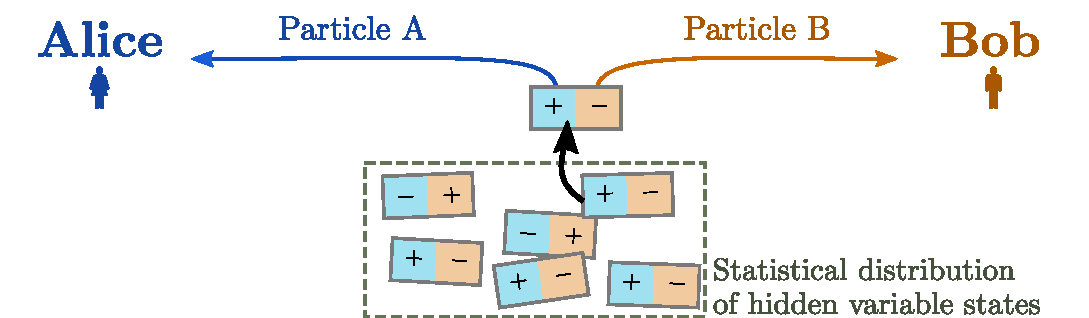
\includegraphics[width=0.75\textwidth]{hiddenvariables}
\end{figure}

When Alice measures $S_z$, the value of the hidden variable is
revealed.  A result of $+z$ implies $\hvbox[+]{-}$, whereas $-z$
implies $\hvbox[-]{+}$.  When Bob subsequently measures $S_z$, his
result is the opposite of Alice's.  But those values were present all
along---no instantaneous physical influence travels between their two
laboratories.

Clearly, there are many missing details in this hypothetical
description.  Any actual hidden variable theory would also need to
replicate the huge list of successful predictions made by quantum
theory.  Trying to come up with a suitable theory of this sort seems
difficult, but with enough hard work, one might imagine that it is
doable.

\section{Bell's theorem}
\label{sec:bell}

In 1964, John S.~Bell published a bombshell paper showing that the
predictions of quantum theory are \textit{inherently inconsistent}
with hidden variable theories [\ref{cite:bell}].  The amazing thing
about this result, known as \textbf{Bell's theorem}, is that it
requires no knowledge about the details of the hidden variable theory,
just that it is deterministic and local.  Here, we present a
simplified version of the theorem due to Mermin [\ref{cite:mermin}].

Suppose once again that we have spin-1/2 particle pairs, with particle
$A$ sent to Alice, and particle $B$ to Bob.  In the framework of
quantum mechanics, particle pairs are repeatedly prepared in the
singlet state
\begin{equation}
  |\psi\rangle = \frac{1}{\sqrt{2}} \Big(|\!+\!z\rangle|\!-\!z\rangle \,-\, |\!-\!z\rangle|\!+\!z\rangle\Big).
  \label{bellsinglet}
\end{equation}
During each round of the experiment, Alice and Bob are each allowed to
measure their particle's spin along one of three possible spin axes,
whose observables are denoted by $S_1$, $S_2$, $S_3$ (we'll specify
the directions of these spin axes later).  Each experimentalist
chooses $S_1$, $S_2$, or $S_3$, \textit{randomly and with equal
  probabilities}.

Many rounds of the experiment are conducted.  After each round, we
record each experimentalist's choice of spin axis and measurement
result ($+$ or $-$), like this:

\begin{figure}[h]
  \centering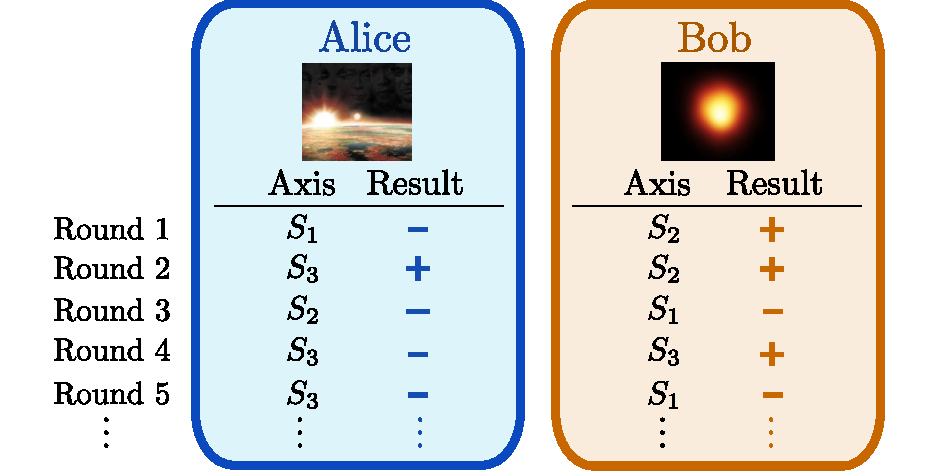
\includegraphics[width=0.67\textwidth]{bell}
\end{figure}

Finally, the experimental records are brought together and examined.
We will assume that the results are consistent with the predictions of
quantum theory.  Among other things, this means that whenever the
experimentalists happened to choose the same axis, their measurement
results have opposite signs.  For instance, in the above example, this
occurred during Round 4, where both experimentalists chose axis $S_3$.

Can a hidden variable theory reproduce the results of quantum theory?
In such a theory, each particle has a definite value for each spin
observable.  For example, particle $A$ might have $S_1 = +\hbar/2, \,
S_2 = +\hbar/2, \, S_3 = -\hbar/2$, which we can express more
concisely just using the signs of the spins: $+, +, -$.  To be
consistent with the predictions of quantum theory for the singlet
state \eqref{bellsinglet}, the two particles' hidden spin variables
must have opposite values for each axis.  Hence, there are $8$
possible ``hidden variable states'', which we denote as follows:
\begin{align*}
  \begin{aligned}
    \hvbox[+++]{---} \;\;\;
    \hvbox[++-]{--+} \;\;\;
    \hvbox[+-+]{-+-} \;\;\;
    \hvbox[+--]{-++}\\
    \hvbox[-++]{+--} \;\;\;
    \hvbox[-+-]{+-+} \;\;\;
    \hvbox[--+]{++-} \;\;\;
    \hvbox[---]{+++}
  \end{aligned}
\end{align*}
For instance, $\hvbox[++-]{--+}$ indicates that for particle $A$, $S_1
= S_2 = +\hbar/2$ and $S_3 = -\hbar/2$, while particle $B$ has $S_1 =
S_2 = -\hbar/2$ and $S_3 = +\hbar/2$.  Instead of the system being
prepared in the quantum state \eqref{bellsinglet}, before each round
the hidden variable state is set to one of the 8 above possibilities,
according to some set of unknown probabilities
\begin{equation*}
  \Big\{ P\big(\hvbox[+++]{---}\,\big), \;P\big(\hvbox[++-]{--+}\,\big),
  \dots, P\big(\hvbox[---]{+++}\,\big) \Big\}.
\end{equation*}

Let us focus on the rounds in which Alice and Bob \textit{chose
  different spin axes}.  Within this subset, what is the probability
\textit{for their measurement results to have opposite signs} (i.e.,
one $+$ and one $-$)?  To answer this question, we first consider
these 6 hidden variable states:
\begin{align*}
  \begin{aligned}
    \hvbox[++-]{--+} \;\;\;
    \hvbox[+-+]{-+-} \;\;\;
    \hvbox[+--]{-++}\\
    \hvbox[-++]{+--} \;\;\;
    \hvbox[-+-]{+-+} \;\;\;
    \hvbox[--+]{++-}
  \end{aligned}
\end{align*}
These are the cases for which each particle's spin variables are not
all $+$ or all $-$.  Take the first case, $\hvbox[++-]{--+}$.  Under
our assumption that Alice and Bob chose different measurement axes,
there are two choices that give opposite signs for the measurement
results: $(S_1,S_2)$ or $(S_2,S_1)$.  Conversely, there are four
choices that give the same sign: $(S_1,S_3)$, $(S_2,S_3)$, $(S_3,S_1)$
and $(S_3, S_2)$.  Since the axis choices are totally random, the
probability of obtaining opposite signs for this hidden variable state
is 1/3.  Going through the rest of the 6 hidden variable states listed
above, we find that the probability to get opposite signs is likewise
1/3.  In the notation of conditional probabilities,
\begin{equation}
  P\big(\textrm{opp.} | \hvbox[++-]{--+}\,\big) =
  P\big(\textrm{opp.} | \hvbox[+-+]{-+-}\,\big) = \cdots = \frac{1}{3},
  \label{bell1}
\end{equation}
where ``opp.''~stands for opposite signs being obtained in the two
measurement results.

Now look at the remaining 2 hidden variable states:
\begin{equation*}
    \hvbox[+++]{---} \;\;\;
    \hvbox[---]{+++}
\end{equation*}
For these, the conditional probabilities are evidently
\begin{equation}
  P\big(\textrm{opp.} | \hvbox[+++]{---}\,\big) =
  P\big(\textrm{opp.} | \hvbox[---]{+++}\,\big) = 1.
  \label{bell2}
\end{equation}
By the law of conditional probabilities, the probability for the
``opposite signs'' outcome is
\begin{align}
  \begin{aligned}
    P\big(\textrm{opp.}\big) &= \;\;\;
    P\big(\textrm{opp.} | \hvbox[++-]{--+}\,\big)
    P\big(\hvbox[++-]{--+}\,\big) \\
    &\quad+ P\big(\textrm{opp.} | \hvbox[+-+]{-+-}\,\big)
    P\big(\hvbox[+-+]{-+-}\,\big) \\
    &\quad+ \quad \cdots \\
    &\quad+ P\big(\textrm{opp.} | \hvbox[---]{+++}\,\big)
    P\big(\hvbox[---]{+++}\,\big),
  \end{aligned}
\end{align}
where the sum runs over all 8 possibilities (hidden variable states).
We can use Eqs.~\eqref{bell1} and \eqref{bell2} to insert the
conditional probabilities, resulting in
\begin{align}
  \begin{aligned}
    P\big(\textrm{opp.}\big) &=
    \frac{1}{3} \Big[\underbrace{P\big(\hvbox[++-]{--+}\,\big)
      + P\big(\hvbox[+-+]{-+-}\,\big)
      + \cdots + P\big(\hvbox[--+]{++-}\,\big)}_{\textrm{6 hidden variable states
obeying Eq.~\eqref{bell1}}}\Big] \\
    &\quad + \underbrace{P\big(\hvbox[+++]{---}\,\big)
    + P\big(\hvbox[---]{+++}\,\big)}_{\textrm{2 hidden variable states obeying \eqref{bell2}}}.
  \end{aligned}
\end{align}
It follows that
\begin{equation}
  P\big(\textrm{opp.}\big) \ge
  \frac{1}{3} \Big[\underbrace{P\big(\hvbox[++-]{--+}\,\big)
      + \cdots + P\big(\hvbox[---]{+++}\,\big)}_{\textrm{all 8 hidden variable states}}
    \Big]
  \label{bellprob}
\end{equation}
The probabilities---whatever they are---must sum to one, so
\begin{equation}
  P\big(\textrm{opp.}\big) \ge \frac{1}{3}.
  \label{bellresult}
\end{equation}
This result, called \textbf{Bell's inequality}, can be summarized as
follows:

\begin{framed}
\noindent
\textit{In a hidden variable theory, for the rounds where Alice and
  Bob choose different spin axes, their measurement results have
  opposite signs with probability $\ge 1/3$.}
\end{framed}

If we can identify a situation where quantum theory predicts a
probability $P < 1/3$, violating Bell's inequality, that would prove
that quantum theory is fundamentally inconsistent with a general class
of hidden variable theories.  It would not matter how complicated the
``inner workings'' of the hidden variable theory may be, so long as it
meets the modest assumptions in the above derivation---e.g., that
there are local deterministic hidden variables that specify each
measurement outcome, and that the occurrences of the hidden variable
states in each round are associated with probabilities that sum to
one.

To complete the proof, we must find a set $\{S_1, S_2, S_3\}$ such
that the predictions of quantum mechanics violate Bell's inequality.
One simple choice is to align $S_1$ with the $z$ axis, and align $S_2$
and $S_3$ along the $x$-$z$ plane at $120^\circ$ ($2\pi/3$ radians)
from $S_1$, as shown below:

\begin{figure}[h]
  \centering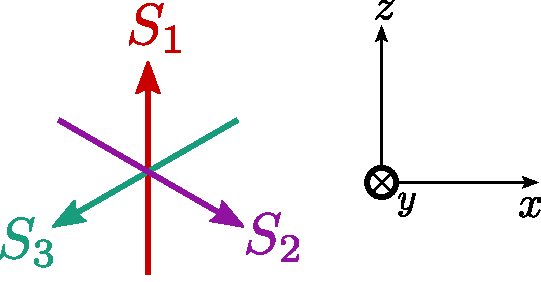
\includegraphics[width=0.28\textwidth]{bellaxes}
\end{figure}

The corresponding spin operators can be written in the eigenbasis of
$\hat{S}_z$:
\begin{align}
  \begin{aligned}\hat{S}_1 &= \frac{\hbar}{2} \, \sigma_3 \\ \hat{S}_2 &= \frac{\hbar}{2} \, \left[\cos(2\pi/3) \sigma_3 + \sin(2\pi/3)\sigma_1\right]  \\   \hat{S}_3 &= \frac{\hbar}{2} \, \left[\cos(2\pi/3) \sigma_3 - \sin(2\pi/3)\sigma_1\right].\end{aligned}
\end{align}

Suppose Alice chooses $S_1$, and obtains $+\hbar/2$.  Particle $A$
collapses to state $|\!+\!z\rangle$, and particle $B$ collapses to
state $|\!-\!z\rangle$.  Bob is assumed to choose a different spin
axis.  If the choice is $S_2$, the expectation value is
\begin{align}
  \begin{aligned}\langle\, - z \, | \, S_2 \,|-\!z\,\rangle &= \frac{\hbar}{2} \Big[\cos(2\pi/3) \langle\,- z\,|\sigma_3| - \!z\,\rangle + \sin(2\pi/3)\langle\,- z\,|\sigma_1|-\!z\,\rangle\Big]\\ &= \frac{\hbar}{2} \cdot \frac{1}{2} \end{aligned}
\end{align}
If $P_+$ and $P_-$ respectively denote the probability of measuring
$+\hbar/2$ and $-\hbar/2$ in this measurement, the above equation
implies that $P_+ - P_- = + 1/2$.  Moreover, $P_+ + P_- = 1$ by
probability conservation.  Hence, the probability of obtaining a
negative value (the opposite sign from Alice's measurement) is $P_- =
1/4$.  All the other possible scenarios are worked out similarly.  The
result is that the overall probability of the two experimentalists
obtaining opposite results (in the cases where they choose different
measurement axis) is $1/4$.  Bell's inequality is violated!

Last of all, we must consult Nature.  Is it possible to experimentally
observe a violation of Bell's inequality?  In the decades following
Bell's paper, many experiments were performed to answer this question.
These experiments are all substantially more complicated than the
above toy model, and are subject to various real-world imperfections.
But in the end, the experimental consensus is a clear \textit{yes}:
Nature agrees with quantum mechanics, not the hidden variable
theories!  The experimental evidence is reviewed in a paper by Aspect
[\ref{cite:aspect}].

\section{Quantum cryptography}

One of the most remarkable consequences of Bell's thought experiment
is that it provides a way to perform cryptography that is more secure,
in certain respects, than conventional cryptography.  The possibility
of \textbf{quantum cryptography} is poised to be one of the most
important technological applications of quantum mechanics.  Here, we
describe one of the earliest quantum cryptography schemes, devised by
Ekert in 1991 [\ref{cite:ekert}].

Ekert's scheme allows two participants, Alice and Bob, to share with
each other a string of random binary digits (0 or 1), called a
``key''.  The objective is to make this sharing secure, in the sense
that no one else can eavesdrop and learn the key.  After Alice and Bob
have established the key, they can use it alongside various
non-quantum methods to encrypt messages between each other (e.g., by using the key as a
\href{https://en.wikipedia.org/wiki/One-time_pad}{one-time pad}).

The scheme follows almost immediately from the Bell thought experiment
of Section \ref{sec:bell}.  In each round, a pair of spin-$1/2$
particles is prepared in the singlet state, with particle $A$ sent to
Alice and $B$ sent to Bob.  Alice and Bob each randomly choose a
measurement axis ($S_1$, $S_2$, or $S_3$) to measure the spin of their
particle.

After many rounds, Alice and Bob publicly announce their choices of
measurement axes.  These announcements are assumed to take place over
some communication channel that cannot be jammed or manipulated by any
hostile party---but \textit{can} be eavesdropped upon.  Next, Alice
and Bob locate the rounds in which they picked the same axis (about
1/3 of the rounds).  Their results for these rounds must be the
opposites of each other.  Hence, they have established a random binary
string known to each other but to no one else.

How might a third party, Eve, attempt to eavesdrop?  Suppose Eve can
intercept some or all of the $B$ particles intended for Bob.  She
might try to extract information from these particles---which, in
quantum theory, means doing measurements on them---and sending along
replacement particles to Bob, hoping he does not notice.  However,
such measurements would break the entanglement between the particles
received by Alice and Bob.  The situation turns into a kind of hidden
variable theory, with the ``hidden variables'' corresponding to the
information extracted by Eve.  To check for this, Alice and Bob can
announce their measurement results for the rounds in which they chose
different axes (as those rounds are not needed for the secret key),
and determine whether Bell's inequality is violated (which would mean
that no eavesdropping has taken place).  For details, refer to
Ref.~[\ref{cite:ekert}].

Alternatively, Eve might try to ``clone'' the quantum state of
particle $B$ before passing it along to Bob.  If this can be done, Eve
can retain the cloned quantum state, wait for Bob to announce his
choice of measurement axis for that round, and then perform the
corresponding measurement to reproduce Bob's result.  Though plausible
at first glance, this turns out to be incompatible with the laws of
quantum mechanics.

The so-called \textbf{no-cloning theorem} can be proven as follows.
Eve desires to clone an arbitrary state of a spin-half particle $B$
onto another spin-half particle $C$.  The two-particle Hilbert space
is $\mathscr{H}\otimes\mathscr{H}$.  With particle $C$ initially
prepared in some state $|0\rangle$, Eve must devise a unitary
operation $\hat{U}$, representing the cloning process, such that
\begin{equation}
  \hat{U} |\psi\rangle | 0\rangle = e^{i\phi} |\psi\rangle |\psi\rangle
  \label{clone}
\end{equation}
for all $|\psi\rangle \in \mathscr{H}$.  The phase factor $\phi$ can
depend on $|\psi\rangle$.

Now replace $|\psi\rangle$ in the above equation with two arbitrary
states denoted by $|\psi_1\rangle$ and $|\psi_2\rangle$, and take
their inner product.  According to Eq.~\eqref{clone},
\begin{align}
  \Big(\langle \psi_1 | \langle 0 | \hat{U}^\dagger \Big)
  \Big(\hat{U} | \psi_2 \rangle |0\rangle \Big)
  &=  \Big(\langle \psi_1| \langle \psi_1| e^{-i\phi_1} \Big) \Big( e^{i\phi_2} |\psi_2\rangle|\psi_2\rangle\Big) \\
  &= e^{-i(\phi_1-\phi_2)} \Big( \langle\psi_1 | \psi_2\rangle \Big)^2. \label{clone1}
\end{align}
Here, $\phi_1$ and $\phi_2$ are the phase factors from
Eq.~\eqref{clone} for the two chosen states.  On the other hand, since
$\hat{U}$ is unitary,
\begin{align}
  \langle \psi_1 | \langle 0 | \hat{U}^\dagger \hat{U} | \psi_2 \rangle |0\rangle
  &= \Big(\langle \psi_1 | \langle 0| \Big) \Big(| \psi_2 \rangle |0\rangle\Big)
  \\ &= \langle\psi_1 | \psi_2\rangle. \label{clone2}
\end{align}
Comparing the magnitudes of \eqref{clone1} and \eqref{clone2},
\begin{equation}
  \big|\langle \psi_1 | \psi_2\rangle \big|^2
  = \big| \langle\psi_1 | \psi_2\rangle \big|
  \;\;\Rightarrow \;\;
  \big|\langle\psi_1 | \psi_2\rangle\big| = 0 \;\mathrm{or}\; 1.
\end{equation}
But aside from the trivial case of a one-dimensional Hilbert space,
this cannot be true for arbitrary $|\psi_1\rangle$ and
$|\psi_2\rangle$.  For instance, for a two-dimensional space spanned
by an orthonormal basis $\{|0\rangle, |1\rangle\}$, we can pick
\begin{equation}
  |\psi_1\rangle = |0\rangle, \;
  |\psi_2\rangle = \frac{1}{\sqrt{2}}\big(|0\rangle +
  |1\rangle\big)
  \;\;\Rightarrow\;\;
  \big|\langle\psi_1|\psi_2\rangle\big| = \frac{1}{\sqrt{2}}.
\end{equation}

\section{Density operators}

We now introduce the \textbf{density operator}, which helps to
streamline many calculations in multi-particle quantum mechanics.

Consider a quantum system with a $d$-dimensional Hilbert space
$\mathscr{H}$.  Given an arbitrary state $|\psi\rangle \in
\mathscr{H}$, define
\begin{equation}
  \hat{\rho} = |\psi\rangle\, \langle\psi|.
  \label{rho_pure}
\end{equation}
This is just the projection operator for $|\psi\rangle$, but in this
context we call it a ``density operator''.  Some other authors call it
a \textbf{density matrix}, based on the fact that linear operators can
be represented as matrices.  It has the following noteworthy features:

\begin{enumerate}
\item It is Hermitian.  

\item Suppose $\hat{Q}$ is an observable with eigenvalues $\{q_\mu\}$
  and eigenstates $\{|\mu\rangle\}$ (where $\mu$ is some label that
  enumerates the eigenstates.  If we do a $\hat{Q}$ measurement on
  $|\psi\rangle$, the probability of obtaining $q_\mu$ is
  \begin{equation}
    P_\mu = \big|\langle \mu | \psi\rangle\big|^2 =
    \langle \mu |\, \hat{\rho}\, | \mu \rangle.
    \label{Pi_rho}
  \end{equation}

\item Moreover, the expectation value of the observable is
  \begin{equation}
    \langle Q\rangle
    = \sum_\mu q_\mu P_\mu
    = \sum_\mu q_\mu \langle \mu | \hat{\rho}| \mu \rangle
    = \mathrm{Tr}\big[\,\hat{Q} \, \hat{\rho}\,\big].
    \label{Qexpt}
  \end{equation}
  In the last equality, $\mathrm{Tr}[\cdots]$ denotes the trace, which
  is the sum of the diagonal elements of the matrix representation of
  the operator.  The value of the trace is basis-independent.
\end{enumerate}

Now consider, once again, a composite system consisting of two
subsystems $A$ and $B$, with Hilbert spaces $\mathscr{H}_A$ and
$\mathscr{H}_B$.  Let's say we are interested in the physical behavior
of $A$, that is to say the outcome probabilities and expectation
values of any measurements performed on $A$.  These can be calculated
from $|\psi\rangle$, the state of the combined system; however,
$|\psi\rangle$ also carries information about $B$, which is not
relevant to us as we only care about $A$.

There is a more economical way to encode just the information about
$A$.  We can define the density operator for subsystem $A$ (sometimes
called the \textbf{reduced density operator}):
\begin{equation}
  \hat{\rho}_A = \mathrm{Tr}_B \,\big[\,\hat{\rho}\,\big].
  \label{rhoa_def}
\end{equation}
Here, $\mathrm{Tr}_B[\cdots]$ refers to a \textbf{partial trace}.
This means tracing over the $\mathscr{H}_B$ part of the Hilbert space
$\mathscr{H} = \mathscr{H}_A \otimes \mathscr{H}_B$, which yields an
operator acting on $\mathscr{H}_A$.

To better understand Eq.~\eqref{rhoa_def}, let us go to an explicit
basis.  Let $\hat{Q}_A$ be an observable for $\mathscr{H}_A$ with
eigenbasis $\{|\mu\rangle\}$, and let $\hat{Q}_B$ be an observable for
$\mathscr{H}_B$ with eigenbasis $\{|\nu\rangle\}$.  If the density
operator of the combined system is $\hat{\rho} = |\psi\rangle\langle
\psi|$, then
\begin{equation}
  \hat{\rho}_A =
    \sum_\nu
    \Big( \hat{I}\otimes \langle \nu| \Big)
    \; |\psi\rangle \langle \psi | \;
    \Big( \hat{I}\otimes | \nu\rangle \Big).
    \label{rhoa_explicit}
\end{equation}
This is a Hermitian operator acting on the $\mathscr{H}_A$ space.  In
the $\{|\mu\rangle\}$ basis, its diagonal matrix elements are
\begin{align}
  \begin{aligned}
    \langle \mu | \hat{\rho}_A | \mu \rangle
    &=
    \sum_\nu
    \Big( \langle \mu| \langle \nu| \Big)
    \, |\psi\rangle \langle \psi | \,
    \Big( |\mu\rangle | \nu\rangle \Big) \\
    &=
    \langle \psi | \,
    \left[ |\mu\rangle \langle \mu| \otimes
      \left(\sum_\nu | \nu\rangle \langle \nu|\right) \right]
    |\psi\rangle \\
    &=
    \langle \psi | \,
    \Big( |\mu\rangle \langle \mu| \otimes \hat{I}_B\Big) |\psi\rangle.
  \end{aligned}
\end{align}
According to the rules of partial measurements discussed in
Section~\ref{sec:partialmeasurements}, this is precisely the
probability of obtaining $q_\mu$ when measuring $\hat{Q}_A$ on subsystem
$A$:
\begin{equation}
  P_\mu = \langle \mu | \hat{\rho}_A | \mu \rangle.
  \label{rho_prob}
\end{equation}
It follows that the expectation value for observable $\hat{M}$ is
\begin{equation}
  \langle Q_A \rangle = \sum_\mu q_\mu
  \langle \mu | \hat{\rho}_A | \mu \rangle
  = \mathrm{Tr}\Big[\hat{Q}_A \, \hat{\rho}_A \Big].
  \label{rho_expect}
\end{equation}
These results hold for any choice of basis.  Hence, knowing the
density operator for $A$, we can determine the outcome probabilities
of \textit{any} partial measurement performed on $A$.

To better understand the properties of $\hat{\rho}_A$, let us write
$|\psi\rangle$ explicitly as
\begin{equation}
  |\psi\rangle = \sum_{\mu\nu} \psi_{\mu\nu} |\mu\rangle |\nu\rangle,
\end{equation}
where $\sum_{\mu\nu} |\psi_{\mu\nu}|^2 = 1$.  Then
\begin{align}
  \begin{aligned}
    \hat{\rho} &= \sum_{\mu\mu'\nu\nu'} \psi_{\mu\nu}
    \psi_{\mu'\nu'}^* \; |\mu\rangle |\nu\rangle \,
    \langle\mu'|\langle \nu'| \\
    \hat{\rho}_A &= \sum_{\mu\mu'\nu} \psi_{\mu\nu}\psi_{\mu'\nu}^* |\mu\rangle
    \langle\mu'| \\
    &= \sum_\nu \left(\sum_\mu \psi_{\mu\nu} |\mu\rangle\right)
    \left(\sum_{\mu'} \psi_{\mu'\nu}^*\langle\mu'|\right) \\
    &= \sum_\nu |\varphi_\nu\rangle \langle \varphi_\nu|,
    \;\;\;\mathrm{where}\;\;\;
    |\varphi_\nu\rangle = \sum_\mu \psi_{\mu\nu} |\mu\rangle.
  \end{aligned}
\end{align}
But $|\varphi_\nu\rangle$ is not necessarily normalized to unity:
$\langle \varphi_\nu | \varphi_\nu\rangle =
\sum_{\mu}|\psi_{\mu\nu}|^2 \le 1$.  Let us define
\begin{equation}
  |\tilde{\varphi}_\nu\rangle = \frac{1}{\sqrt{P_\nu}} |\varphi_\nu\rangle,
  \;\;\;\mathrm{where} \;\; P_\nu = \sum_{\mu}|\psi_{\mu\nu}|^2.
\end{equation}
Note that each $P_\nu$ is a non-negative real number in the range
$[0,1]$.  Then
\begin{equation}
  \hat{\rho}_A = \sum_\nu P_\nu\, |\tilde{\varphi}_\nu\rangle
  \langle \tilde{\varphi}_\nu|,
  \;\;\;\mathrm{where}\;\;
  \begin{cases}
    \;\;\textrm{each $P_\nu$ is a real number in $[0,1]$, and} \\
    \;\;\textrm{each}\; |\tilde{\varphi}_\nu\rangle \in \mathscr{H}_A,
    \;\;\mathrm{with}
    \;\;\langle\tilde{\varphi}_\nu|\tilde{\varphi}_\nu\rangle = 1.
  \end{cases}
  \label{rhoform}
\end{equation}

In general, we can define a density operator as any operator that has
the form of Eq.~\eqref{rhoform}, regardless of whether or not it was
formally derived via a partial trace.  We can interpret it as
describing a ensemble of quantum states weighted by a set of classical
probabilities.  Each term in the sum consists of (i) a weighting
coefficient $P_\nu$ which can be regarded as a probability (the
coefficients are all real numbers in the range $[0,1]$, and sum to 1),
and (ii) a projection operator associated with some normalized state
vector $|\tilde{\varphi}_\nu\rangle$.  Note that the states in the
ensemble do not have to be orthogonal to each other.

From this point of view, a density operator of the form
$|\psi\rangle\langle\psi|$ corresponds to the special case of an
ensemble containing only one quantum state $|\psi\rangle$.  Such an
ensemble is called a \textbf{pure state}, and describes a quantum
system that is not entangled with any other system.  If an ensemble is
not a pure state, we call it a \textbf{mixed state}; it describes a
system that is entangled with some other system.

We can show that any linear operator $\hat{\rho}_A$ obeying
Eq.~\eqref{rhoform} has the following properties:
\begin{enumerate}
\item $\hat{\rho}_A$ is Hermitian.

\item $\langle\varphi|\hat{\rho}_A|\varphi\rangle \ge 0$ for any
  $|\varphi\rangle \in \mathscr{H}_A$ (i.e., the operator is positive
  semidefinite).

\item For any observable $\hat{Q}_A$ acting on $\mathscr{H}_A$,
  \begin{align}
    \begin{aligned}
      \langle Q_A \rangle
      &\equiv \sum_\nu P_\nu
      \langle \tilde{\varphi}_\nu|\hat{Q}_A|\tilde{\varphi}_\nu\rangle \\
      &= \sum_{\mu\nu} P_\nu\,
      \langle \tilde{\varphi}_\nu|\mu\rangle \,
      \langle\mu|\hat{Q}|\tilde{\varphi}_\nu\rangle
      \;\;\;\big(\textrm{using some basis} \;\{|\mu\rangle\}\big) \\
      &= \sum_\mu
      \langle\mu|\hat{Q} \left(\sum_\nu |\tilde{\varphi}_\nu\rangle
      \langle \tilde{\varphi}_\nu|\right) |\mu\rangle \\
      &= \mathrm{Tr}\left[\,\hat{Q} \,\hat{\rho}_A\,\right].
    \end{aligned}
    \label{prop3}
  \end{align}
  This property can be used to deduce the probability of obtaining any
  measurement outcome: if $|\mu\rangle$ is the eigenstate associated
  with the outcome, the outcome probability is
  $\langle\mu|\hat\rho_A|\mu\rangle$, consistent with
  Eq.~\eqref{rho_prob}.  To see this, take $\hat{Q} = |\mu\rangle
  \langle \mu|$ in Eq.~\eqref{prop3}.
  
\item The eigenvalues of $\hat{\rho}_A$, denoted by $\{p_1, p_2,
  \dots, p_{d_A}\}$, satisfy
  \begin{equation}
    p_j \in \mathbb{R} \;\;\;\mathrm{and}\;\; 0 \le p_j \le 1 \;\;
    \mathrm{for}\;\; j = 1,\dots,d_A,
    \quad\mathrm{with}\;\; \sum_{j=1}^{d_A} p_j = 1.
    \label{trrho_reduced}    
  \end{equation}
  The eigenvalues can thus be interpreted as probabilities.  Moreover,
  $\mathrm{Tr}[\hat\rho_A] = 1$.

  Property 4 follows from Property 3.  First, take $\hat{Q} =
  |j\rangle\langle j|$, where $|j\rangle$ is any eigenvector of
  $\hat\rho_A$ with eigenvalue $p_j$, and use Property 3 to prove that
  $0 \le p_j \le 1$.  Then take $\hat{Q} = \hat{I}_A$ and use Property
  3 to prove that the eigenvalues sum to 1.
\end{enumerate}

\section{Entanglement entropy}
\label{sec:entropy}

Previously, we said that a multi-particle system is entangled if the
individual particles lack definite quantum states.  It would be nice
to make this statement more precise, and in fact physicists have come
up with several different quantitive measures of entanglement.  In
this section, we will describe the most common measure,
\textbf{entanglement entropy}, which is closely related to the entropy
concept from thermodynamics, statistical mechanics, and information
theory.

We have seen from the previous section that if a subsystem $A$ is
(possibly) entangled with some other subsystem $B$, the information
required to calculate all partial measurement outcomes on $A$ is
stored within a reduced density operator $\hat{\rho}_A$.  We can use
this to define a quantity called the \textbf{entanglement entropy} of
$A$:
\begin{equation}
  S_{A} = - k_b \, \mathrm{Tr}_A \Big\{ \hat{\rho}_A\, \ln\!\big[\hat{\rho}_A\big]\Big\}.
  \label{entropy}
\end{equation}
In this formula, $\ln[\cdots]$ denotes the logarithm of an operator,
which is the inverse of the exponential: $\ln(\hat{P}) = \hat{Q}
\Rightarrow \exp(\hat{Q}) = \hat{P}$.  The prefactor $k_b$ is
Boltzmann's constant, and ensures that $S_A$ has the same units as
thermodynamic entropy.

The definition of the entanglement entropy is based on an analogy with
the entropy concept from classical thermodynamics, statistical
mechanics and information theory.  In those classical contexts,
entropy is a quantitative measure of uncertainty (i.e, lack of
information) about a system's underlying microscopic state, or
``microstate''.  Suppose a system has $W$ possible microstates that
occur with probabilities $\{p_1, p_2, \dots, p_W\}$, satisfying
$\sum_i p_i = 1$.  Then we define the classical entropy
\begin{equation}
  S_{\mathrm{cl.}} = - k_b \sum_{i=1}^W p_i \ln(p_i).
\end{equation}
In a situation of complete certainty where the system is known to be
in a specific microstate $k$ ($p_i = \delta_{ik}$), the formula gives
$S_{\mathrm{cl.}} = 0$.  (Note that $x \ln(x)\rightarrow 0$ as
$x\rightarrow 0$).  In a situation of complete uncertainty where all
microstates are equally probable ($p_i = 1/W$), we get
$S_{\mathrm{cl.}} = k_b \ln W$, the entropy of a microcanonical
ensemble in statistical mechanics.  For any other distribution of
probabilities, it can be shown that the entropy lies between these two
extremes: $0 \le S_{\mathrm{cl.}}  \le k_b\ln W$.  For a review of the
properties of entropy, see Appendix C.

The concept of entanglement entropy aims to quantify the uncertainty
arising from a quantum (sub)system's lack of a definite quantum state,
due to it being possibly entangled with another (sub)system.  When
formulating it, the key issue we need to be careful about is how to
extend classical notions of probability to quantum systems.  We have
seen that when performing a measurement on $A$ whose possible outcomes
are $\{q_\mu\}$, the probability of getting $q_\mu$ is $P_\mu =
\langle \mu | \hat{\rho}_A|\mu\rangle$.  However, it is problematic to
directly substitute these probabilities $\{P_\mu\}$ into the classical
entropy formula, since they are basis-dependent (i.e., the set of
probabilities is dependent on the choice of measurement).
Eq.~\eqref{entropy} bypasses this problem by using the trace, which is
basis-independent.

In the special case where $\{|\mu\rangle\}$ is the eigenbasis for
$\hat{\rho}_A$, the connection is easier to see.  From
\eqref{trrho_reduced}, the eigenvalues $\{p_\mu\}$ are all real numbers
between 0 and 1, and summing to unity, so they can be regarded as
probabilities.  Then the entanglement entropy is
\begin{align}
  \begin{aligned}
    S_A &= -k_b \sum_\mu \langle \mu | \hat{\rho}_A \ln(\hat{\rho}_A) | \mu\rangle  \\
    &= - k_b \sum_\mu p_\mu \ln(p_\mu).
  \end{aligned}
\end{align}
Therefore, in this particular basis the expression for the
entanglement entropy is consistent with the classical definition of
entropy, with the eigenvalues of $\hat{\rho}_A$ serving as the
relevant probabilities.

By analogy with the classical entropy formula (see Appendix C), the
entanglement entropy has the following bounds:
\begin{equation}
  0 \le S_A \le k_b\ln(d_A),
  \label{Sabounds}
\end{equation}
where $d_A$ is the dimension of $\mathscr{H}_A$.

The lower bound $S_A = 0$ holds if and only if system $A$ is in a pure
state (i.e., it is not entangled with any other system).  This is
because the bound corresponds to a situation where $\hat{\rho}_A$ has
one eigenvalue that is 1, and all the other eigenvalues are 0 (see
Appendix C).  If we denote the eigenvector associated with the
non-vanishing eigenvalue by $|\psi\rangle$, then the density matrix
can be written as $\hat{\rho}_A = |\varphi\rangle\langle\varphi|$, which
has the form of a pure state.

As a corollary, if we find that $S_{A} \ne 0$, then $\hat{\rho}_A$
cannot be written as a pure state $|\psi\rangle\langle\psi|$ for
\textit{any} $|\psi\rangle$, and hence it must describe a mixed state.

A system is said to be \textbf{maximally entangled} if it saturates
the upper bound of \eqref{Sabounds}, $S_A = k_b \ln(d_A)$.  This
occurs if and only if the eigenvalues of the density operator are all
equal: i.e., $p_j = 1/d_A$ for all $j = 1, \dots, d_A$.

\begin{framed}
\noindent
\textit{Example}---Consider the following state of two spin-$1/2$
particles:
\begin{align}
  |\psi\rangle = \frac{1}{\sqrt{2}} \Big(|\!+\!z\rangle|\!-\!z\rangle \,-\, |\!-\!z\rangle|\!+\!z\rangle\Big).
\end{align}
The density operator for the two-particle system is
\begin{equation}
  \hat{\rho}(\psi) = \frac{1}{2} \Big(|\!+\!z\rangle|\!-\!z\rangle \,-\, |\!-\!z\rangle|\!+\!z\rangle\Big) \Big(\langle+z|\langle-z| \,-\, \langle-z|\langle+z|\Big).
\end{equation}
Tracing over system $B$ (the second slot) yields the reduced density operator
\begin{equation}
  \hat{\rho}_A(\psi) = \frac{1}{2} \Big(|\!+\!z\rangle \langle+z| \,+\, |\!-\!z\rangle \langle-z|\Big).
\end{equation}
This can be expressed as a matrix in the
$\{|\!+z\rangle,|\!-z\rangle\}$ basis:
\begin{equation}
  \hat{\rho}_A(\psi) = \begin{pmatrix}\frac{1}{2} & 0 \\ 0 & \frac{1}{2}\end{pmatrix}.
\end{equation}
Now we can use $\hat{\rho}_A$ to compute the entanglement entropy
\begin{equation}
  S_A = -k_b\mathrm{Tr}\left\{\hat{\rho}_A\ln(\rho_A)\right\} = -k_b\mathrm{Tr}\begin{pmatrix}\frac{1}{2}\ln\left(\frac{1}{2}\right) & 0 \\ 0 & \frac{1}{2}\ln\left(\frac{1}{2}\right)\end{pmatrix} = k_b\ln(2).
\end{equation}
Hence, the particles are maximally entangled.
\end{framed}

\section{The Many Worlds Interpretation}

We conclude this chapter by discussing a set of compelling but
controversial ideas arising from the phenomenon of quantum
entanglement: the \textbf{Many Worlds Interpretation} as formulated by
Hugh Everett [\ref{cite:everett}].

So far, when describing the phenomenon of state collapse, we have
relied on the measurement postulate (see
Section~\ref{sec:partialmeasurements}), which is part of the
\textbf{Copenhagen Interpretation} of quantum mechanics.  This is how
quantum mechanics is typically taught, and how physicists think about
the theory when doing practical, everyday calculations.

However, the measurement postulate has two bad features:

\begin{enumerate}
\item It stands apart from the other postulates of quantum mechanics,
  for it is the only place where randomness (or ``indeterminism'')
  creeps into quantum theory.  The other postulates do not refer to
  probabilities.  In particular, the Schr\"odinger equation
\begin{equation}
  i\hbar\frac{\partial}{\partial t}|\psi(t)\rangle = \hat{H}(t) |\psi(t)\rangle
\end{equation}
is completely deterministic.  If you know $\hat{H}(t)$ and are given
the state $|\psi(t_0)\rangle$ at some time $t_0$, you can in principle
determine $|\psi(t)\rangle$ for all $t$.  This time-evolution consists
of a smooth, non-random rotation of the state vector within its
Hilbert space.  A measurement process, however, has a completely
different character: it causes the state vector to jump
discontinuously to a randomly-selected value.  It is strange that
quantum theory contains two completely different ways for a state to
change.

\item The measurement postulate is silent on what constitutes a
measurement.  Does measurement require a conscious observer?  Surely
not: as Einstein once exasperatedly asked, are we really expected to
believe that the Moon exists only when we look at it?  But if a given
device interacts with a particle, what determines whether it acts via
the Schr\"odinger equation, or performs a measurement?
\end{enumerate}

The Many Worlds Interpretation seeks to resolve these problems by
positing that \textit{the measurement postulate is \underline{not} a
  fundamental postulate of quantum mechanics}.  Rather, what we call
``measurement'', including state collapse and the apparent randomness
of measurement results, is an emergent phenomenon that can be derived
from the behavior of complex many-particle quantum systems obeying the
Schr\"odinger equation.  The key idea is that a measurement process
can be described by applying the Schr\"odinger equation to a quantum
system containing both the thing being measured \textit{and} the
measurement apparatus itself.

We can study this using a toy model formulated by Albrecht
[\ref{cite:albrecht}].  Consider a spin-$1/2$ particle, and an
apparatus designed to measure $S_z$.  Let $\mathscr{H}_S$ be the
spin-$1/2$ Hilbert space (which is 2D), and $\mathscr{H}_A$ be the
Hilbert space of the apparatus (which has dimension $d$).  We will
assume that $d$ is very large, as actual experimental apparatuses are
macroscopic objects containing $10^{23}$ or more atoms!  The Hilbert
space of the combined system is
\begin{equation}
  \mathscr{H} = \mathscr{H}_S \otimes \mathscr{H}_A,
\end{equation}
and is $2d$-dimensional.  Let us suppose the system is prepared in an initial
state
\begin{equation}
  |\psi(0)\rangle = \Big(a_+ |\!+z\rangle + a_- |\!-z\rangle\Big) \otimes |\Psi\rangle,
\end{equation}
where $a_\pm\in\mathbb{C}$ are the quantum amplitudes for the particle
to be initially spin-up or spin-down, and $|\Psi\rangle \in
\mathscr{H}_A$ is the initial state of the apparatus.

The combined system now evolves via the Schr\"odinger equation.  We
aim to show that if the Hamiltonian has the form
\begin{equation}
  \hat{H} = \hat{S}_z \otimes \hat{V},
\end{equation}
where $\hat{S}_z$ is the operator corresponding to the observable
$S_z$, then time evolution has an effect equivalent to the measurement
of $S_z$.

It turns out that we can show this without making any special choices
for $\hat{V}$ or $|\Psi\rangle$.  We only need $d \gg 2$, and for both
$\hat{V}$ and $|\Psi\rangle$ to be ``sufficiently complicated''.  We
choose $|\Psi\rangle$ to be a random state vector, and choose random
matrix components for the operator $\hat{V}$.  The precise generation
procedures will be elaborated on later.  Once we decide on
$|\Psi\rangle$ and $\hat{V}$, we can evolve the system by solving the
Sch\"odinger equation
\begin{equation}
  |\psi(t)\rangle = U(t)|\psi(0)\rangle, \;\;\;\mathrm{where}\;\; \hat{U}(t) = \exp\left[-\frac{i}{\hbar}\hat{H}t\right].
\end{equation}
Because the part of $\hat{H}$ acting on the $\mathscr{H}_S$ subspace
is $\hat{S}_z$, the result necessarily has the following form:
\begin{align}
  \begin{aligned}|\psi(t)\rangle &= \hat{U}(t)\Big(a_+ |\!+\!z\rangle + a_- |\!-\!z\rangle\Big) \otimes |\Psi\rangle \\ &= a_+ |\!+\!z\rangle \otimes |\Psi_+(t)\rangle \;+\; a_- |\!-\!z\rangle \otimes |\Psi_-(t)\rangle. \end{aligned}
\end{align}
Here, $|\Psi_+(t)\rangle$ and $|\Psi_-(t)\rangle$ are apparatus states
that are ``paired up'' with the $|\!+\!z\rangle$ and $|\!-\!z\rangle$
states of the spin-$1/2$ subsystem.  At $t=0$, both
$|\Psi_+(t)\rangle$ and $|\Psi_-(t)\rangle$ are equal to
$|\Psi\rangle$; for $t > 0$, they rotate into different parts of the
state space $\mathscr{H}_A$.  If the dimensionality of $\mathscr{H}_A$
is sufficiently large, and both $\hat{V}$ and $|\Psi\rangle$ are
sufficiently complicated, we can guess (and we will verify numerically) that
the two state vectors rotate into completely different parts of
the state space, so that
\begin{equation}
  \langle\Psi_+(t) | \Psi_-(t)\rangle \approx 0 \;\;\;\textrm{for sufficiently large}\;\; t.
\end{equation}
Once this is the case, the two terms in the above expression for
$|\psi(t)\rangle$ can be interpreted as two decoupled ``worlds''.  In
one world, the spin has a definite value $+\hbar/2$, and the apparatus
is in a state $|\Psi_+\rangle$ (which might describe, for instance, a
macroscopically-sized physical pointer that is pointing to a ``$S_z =
+\hbar/2$'' reading).  In the other world, the spin has a definite
value $-\hbar/2$, and the apparatus has a different state
$|\Psi_-\rangle$ (which might describe a physical pointer pointing to
a ``$S_z = -\hbar/2$'' reading).  Importantly, the $|\Psi_+\rangle$
and $|\Psi_-\rangle$ states are orthogonal, so they can be rigorously
distinguished from each other.  The two worlds are
``weighted'' by $|a_+|^2$ and $|a_-|^2$, which correspond to the
probabilities of the two possible measurement results.

The above description can be tested numerically.  Let us use an
arbitrary basis for the apparatus space $\mathscr{H}_A$; in that
basis, let the $d$ components of the initial apparatus state vector
$|\Psi\rangle$ be random complex numbers:
\begin{align}
  \begin{aligned}
  |\Psi\rangle = \frac{1}{\sqrt{\mathcal{N}}}\, \begin{pmatrix}\Psi_0 \\ \Psi_1 \\ \vdots \\ \Psi_{d-1}
  \end{pmatrix}, \;\; \mathrm{where} \;\; \mathrm{Re}(\Psi_j), \mathrm{Im}(\Psi_j) \sim N(0,1).
  \end{aligned}
\end{align}
In other words, the real and imaginary parts of each complex number
$\Psi_j$ are independently drawn from the the standard normal
(Gaussian) distribution, denoted by $N(0,1)$.  The normalization
constant $\mathcal{N}$ is defined so that $\langle\Psi|\Psi\rangle =
1$.

Likewise, we generate the matrix elements of $\hat{V}$ according to
the following random scheme:
\begin{align}
  \begin{aligned}A_{ij} &\sim u_{ij} + i v_{ij}, \;\;\;\mathrm{where}\;\;u_{ij},v_{ij}\sim N(0,1)\\ \hat{V} &= \frac{1}{2\sqrt{d}} \left(\hat{A} + \hat{A}^\dagger\right).\end{aligned}
\end{align}
This scheme produces a $d\times d$ matrix with random components,
subject to the requirement that the overall matrix be Hermitian.  The
factor of $1/2\sqrt{d}$ is relatively unimportant; it ensures that the
eigenvalues of $\hat{V}$ lie in the range $[-2,2]$, instead of scaling
with $d$ [\ref{cite:edelman}].

The Schr\"odinger equation can now be solved numerically.  The results
are shown below:

\begin{figure}[h]
  \centering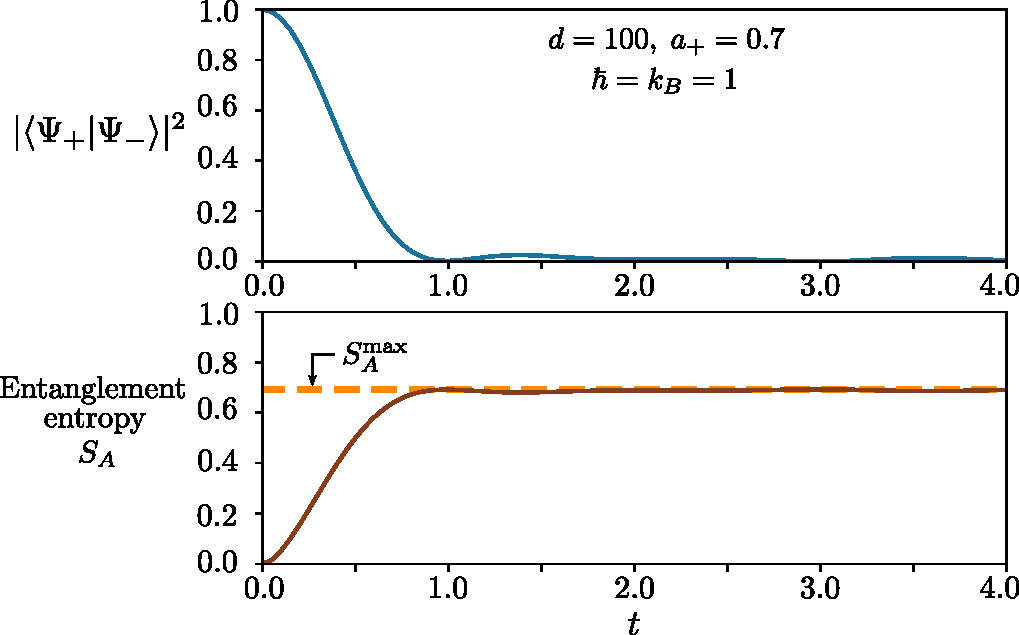
\includegraphics[width=0.7\textwidth]{decoherence}
\end{figure}

In the inital state, we let $a_+ = 0.7$, so $a_- = \sqrt{1-0.7^2} =
0.71414\dots$ The upper panel plots the overlap between the two
apparatus states, $|\langle\Psi_+|\Psi_-\rangle|^2$, versus $t$.  In
accordance with the preceding discussion, the overlap is unity at $t =
0$, but subsequently decreases to nearly zero.  For comparison, the
lower panel plots the entanglement entropy between the two subsystems,
$S_A = -k_b \mathrm{Tr}_A\left\{\hat{\rho}_A\ln\hat{\rho}_A\right\}$,
where $\hat{\rho}_A$ is the reduced density matrix obtained by tracing
over the spin subspace.  We find that $S_A = 0$ at $t=0$, due to the
fact that the spin and apparatus subsystems start out with definite
quantum states in $|\psi(0)\rangle$.  As the system evolves, the
subsystems become increasingly entangled, and $S_A$ increases up to
\begin{equation}
  S_A^{\mathrm{max}}/k_b = - \Big( |a_+|^2 \ln|a_+|^2 + |a_-|^2\ln|a_-|^2 \Big) \approx 0.693
\end{equation}
This value is indicated in the figure by a horizontal dashed line, and
corresponds to the result of the classical entropy formula for
probabilities $\{|a_+|^2,|a_-|^2\}$.  Moreover, we see that the
entropy reaches $S_A^{\mathrm{max}}$ at around the same time that
$|\langle\Psi_+|\Psi_-\rangle|^2$ reaches zero.  This demonstrates the
close relationship between ``measurement'' and ``entanglement''.

For details about the numerical linear algebra methods used to perform
the above calculation, refer to Appendix D.

The ``many worlds'' concept can be generalized from the above toy
model to the universe as a whole.  In the viewpoint of the Many Worlds
Interpretation of quantum mechanics, the entire universe can be
described by a mind-bogglingly complicated quantum state, evolving
deterministically according to the Schr\"odinger equation.  This
evolution involves repeated ``branchings'' of the universal quantum
state, which continuously produces more and more worlds.  The
classical world that we appear to inhabit is just one of a vast
multitude.  It is up to you to decide whether this conception of
reality seems reasonable.  It is essentially a matter of preference,
because the Copenhangen Interpretation and the Many Worlds
Interpretation have identical physical consequences, which is why they
are referred to as different ``interpretations'' of quantum mechanics,
rather than different theories.




\section*{Exercises}

\begin{enumerate}

\item Consider the singlet state
\begin{equation}
  |\psi\rangle = \frac{1}{\sqrt{2}} \Big(|\!+\!z\rangle|\!-\!z\rangle \,-\, |\!-\!z\rangle|\!+\!z\rangle\Big),
\end{equation}
where the left- and right-hand slots refer to subsystems $A$ and $B$
respectively, and $|\pm\!z\rangle$ denotes the eigenstate of the spin
operator $\hat{S}_z$ with eigenvalue $\pm\hbar/2$.
\begin{enumerate}[(a)]
\item Suppose we perform a measurement on $A$ using a rotated spin
  observable
\begin{equation}
  \hat{S}_n = \hat{U}^\dagger \hat{S}_z \hat{U},
\end{equation}
where $\hat{U}$ is a unitary rotation matrix.  The eigenstates of
$\hat{S}_n$ are $|\pm n\rangle = \hat{U}^\dagger |\pm z\rangle$, with
eigenvalues $\pm \hbar/2$.  For each measurement outcome $\pm\hbar/2$,
prove that the collapsed two-particle state is (up to arbitrary phase
and normalization factors)
\begin{equation}
  |\psi'\rangle \propto |\pm \!n \rangle\; |\mp\! n\rangle.
\end{equation}
Hint: you don't need the explicit form of $\hat{U}$, only the fact
that it is unitary.

\item Denote the probabilities of the two outcomes in part (a) by
  $P(A+)$ and $P(A-)$.  Derive expressions for these two
  probabilities.

\item For each of the two outcomes from measuring $S_n$ on $A$, find
  the measurement probabilities for a subsequent $S_z$ measurement on
  $B$, denoted by $P(B_+|A_\pm)$ and $P(B_-|A_\pm)$.  Hence, show that
  \begin{align}
    P(B_+) &= P(B_+|A_+) P(A_+) + P(B_+|A_-) P(A_-) = \frac{1}{2}\\
    P(B_-) &= P(B_-|A_+) P(A_+) + P(B_-|A_-) P(A_-) = \frac{1}{2},
  \end{align}
  regardless of $n$.  Optional: generalize this to any $B$ measurement
  axis.

\end{enumerate}


  
  \label{ex:singletproperties}
  %% \item A vector space $\mathscr{H}$ is said to have an inner product if
%%   there is an pairwise operation between its vectors that satisfies
%%   the following ``inner product axioms''.  For arbitrary
%%   $|\psi\rangle, |\psi'\rangle, |\psi''\rangle \in \mathscr{H}_A$,
%%   \begin{enumerate}
%%   \item $\langle \psi|\psi' \rangle = \langle\psi'|\psi\rangle^*$
%%   \item $\langle \psi|\psi \rangle \in \mathbb{R}^+_0$, and $\langle \psi|\psi \rangle = 0$ if and only if $|\psi\rangle = 0$.
%%   \item $\langle\psi| \, \big(|\psi'\rangle + |\psi'' \rangle\big)
%%     = \langle \psi|\psi'\rangle + \langle \psi|\psi''\rangle$
%%   \item $\langle \psi | \,\big(c|\psi'\rangle\big) = c\langle\psi|\psi'\rangle$ for all $c\in\mathbb{C}$,
%%   \end{enumerate}
%%   Prove that the inner product for $\mathscr{H}_A\otimes\mathscr{H}_B$
%%   defined in Section~\ref{sec:tensorprod} satisfies these axioms.
%%   \label{ex:innerprod}

\item Consider the density operator
  \begin{equation}
    \hat{\rho} = \frac{1}{2} |\!+\!z\rangle \langle+z|
    \,+\, \frac{1}{2} |\!+\!x\rangle \langle+x|
  \end{equation}
  where $|\!+\!x\rangle = \frac{1}{\sqrt{2}} \left(|\!+\!z\rangle +
  |\!-\!z\rangle\right)$.  This can be viewed as an equal-probability
  sum of two different pure states.  However, the density matrix can
  also be written as
  \begin{equation}
    \hat{\rho} \,=\, p_1\, |\psi_1\rangle \langle \psi_1|
    \,+\, p_2\, |\psi_2\rangle \langle\psi_2|
  \end{equation}
  where $|\psi_{1}\rangle$ and $|\psi_{2}\rangle$ are the eigenvectors
  of $\hat{\rho}$.  Show that $p_1$ and $p_2$ are \textit{not} 1/2.
  \label{ex:rho_decomp}


\item 
  Consider two distinguishable particles, $A$ and $B$.  The 2D Hilbert
  space of $A$ is spanned by $\{|m\rangle, |n\rangle\}$, and the
  3D Hilbert space of $B$ is spanned by $\{|p\rangle, |q\rangle,
  |r\rangle\}$.  The two-particle state is
\begin{equation}
  |\psi\rangle = \frac{1}{3} \, |m\rangle|p\rangle
+ \frac{1}{\sqrt{6}} \, |m\rangle|q\rangle
+ \frac{1}{\sqrt{18}} \, |m\rangle|r\rangle
+ \frac{\sqrt{2}}{3} \, |n\rangle|p\rangle
+ \frac{1}{\sqrt{3}} \, |n\rangle|q\rangle
+ \frac{1}{3} \, |n\rangle|r\rangle.
\end{equation}
Find the entanglement entropy.

\end{enumerate}

\section*{Further Reading}

\begin{enumerate}[[1{]}]
\item Bransden \& Joachain, \S14.1---14.4, \S17.1--17.5

\item Sakurai, \S3.9

\item A.~Einstein, B.~Podolsky, and N.~Rosen,
  \textit{Can Quantum-Mechanical Description of Physical Reality Be
    Considered Complete?}, Physical Review \textbf{47}, 777 (1935).
  [\href{https://journals.aps.org/pr/abstract/10.1103/PhysRev.47.777}{link}]
  \label{cite:epr}

\item J.~S.~Bell, \textit{On the Einstein-Podolsky-Rosen paradox},
  Physics \textbf{1}, 195 (1964). [\href{http://inspirehep.net/record/31657/files/}{link}]\label{cite:bell}
  
\item N.~D.~Mermin, \textit{Bringing home the atomic world: Quantum
  mysteries for anybody}, American Journal of Physics \textbf{49}, 940
  (1981). [\href{http://aapt.scitation.org/doi/abs/10.1119/1.12594}{link}] \label{cite:mermin}

\item A.~Aspect, \textit{Bell's inequality test: more ideal than ever},
  Nature (News and Views) \textbf{398}, 189 (1999). [\href{https://www.nature.com/articles/18296}{link}] \label{cite:aspect}

\item A.~K.~Ekert, \textit{Quantum Cryptography Based on Bell's Theorem},
  Physical Review Letters \textbf{67}, 661 (1991). [\href{https://journals.aps.org/prl/abstract/10.1103/PhysRevLett.67.661}{link}] \label{cite:ekert}

  
\item H.~Everett, III, \textit{The Theory of the Universal Wave
  Function} (PhD thesis), Princeton University (1956)
  [\href{http://ucispace.lib.uci.edu/handle/10575/1302}{link}]
\label{cite:everett}

\item A.~Albrecht, \textit{Following a ``collapsing'' wave function},
  Physical Review D \textrm{48}, 3768 (1993). [\href{https://journals.aps.org/prd/abstract/10.1103/PhysRevD.48.3768}{link}]
\label{cite:albrecht}

\item A.~Edelman and N.~R.~Rao, \textit{Random matrix theory}, Acta
  Numerica \textbf{14}, 233 (2005). [\href{https://doi.org/10.1017/S0962492904000236}{link}]
\label{cite:edelman}
\end{enumerate}

\end{document}


%% For decades after the discovery of quantum mechanics, the quantum
%% double-slit experiment was just a ``thought experiment'', meant to
%% illustrate the features of quantum mechanics that had been uncovered
%% by other, more complicated experiments.  Nowadays, the most convenient
%% way to do the experiment is with light, using single-photon sources
%% and single-photon detectors.  Quantum interference has also been
%% demonstrated experimentally using electrons, neutrons, and even
%% large-scale particles such as buckyballs.
